\documentclass[12pt, a4paper]{article}
\usepackage[french]{babel}
\usepackage[utf8]{inputenc}
\usepackage{geometry}
\geometry{top=2.5cm, right=2.5cm, left=2.5cm}
\usepackage{graphicx}
\graphicspath{/images}

\title{Github POMPES -- Figures à demander aux professeurs}

\author{ITBepolytech}
\begin{document}
\maketitle
\section{Anne \textsc{Delandtsheer} -- MATH-H2000 : Analyse II}
\subsection{Chapitre 10 : Analyse vectorielle}
\subsubsection{Figure 10.3 -- Coordonnées polaires}
\begin{center}
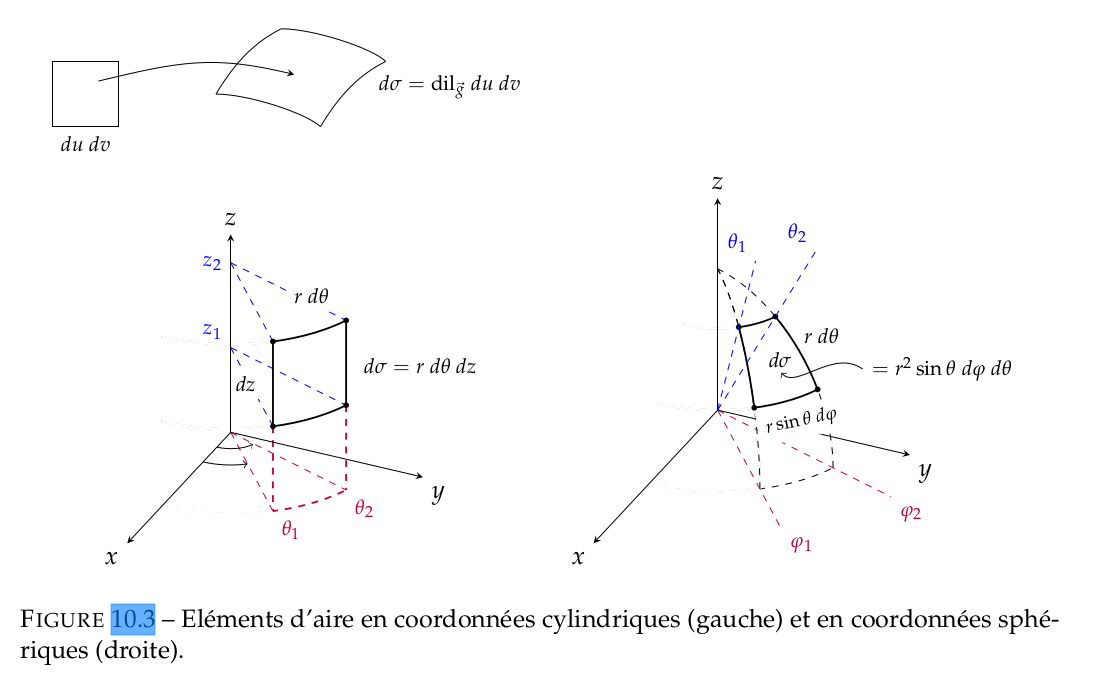
\includegraphics[width=0.9\textwidth]{images/MATH-H2000_10_3}
\end{center}
\subsubsection{Figure 10.10 -- Discrétisation d'une surface}
\begin{center}
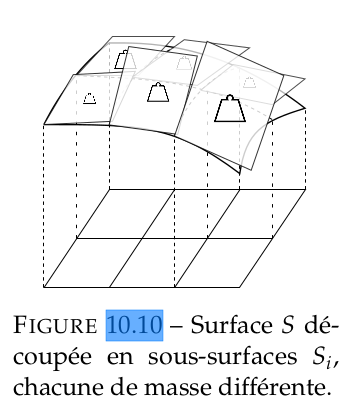
\includegraphics[scale=0.4]{images/MATH-H2000_10_10}
\end{center}
\subsubsection{Figure 10.16 -- Projection d'un parallélogramme}
\begin{center}
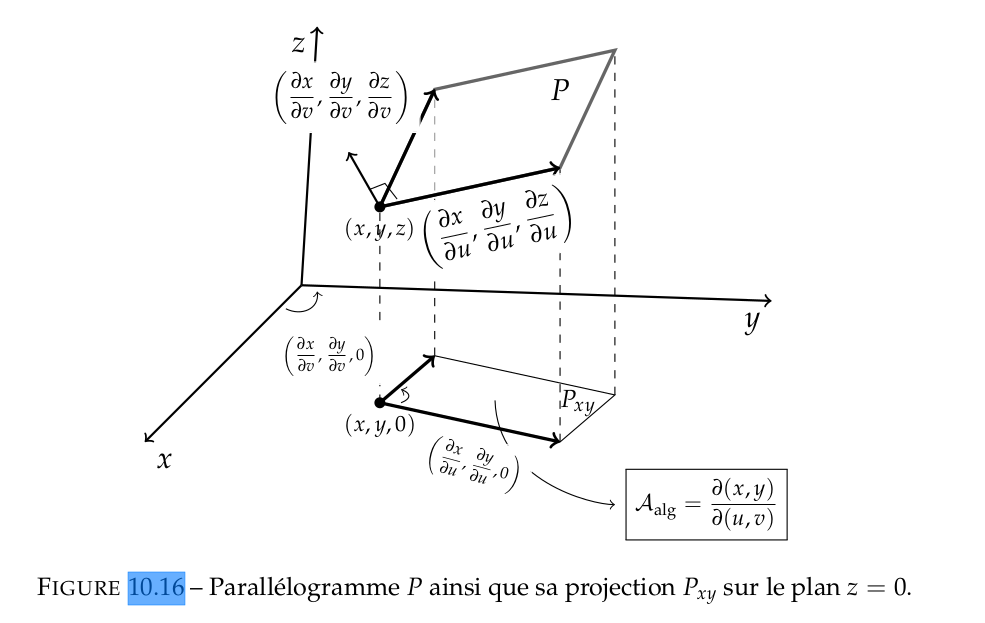
\includegraphics[scale=0.4]{images/MATH-H2000_10_16}
\end{center}
\subsubsection{Figure 10.17 -- Décomposition d'un flux}
\begin{center}
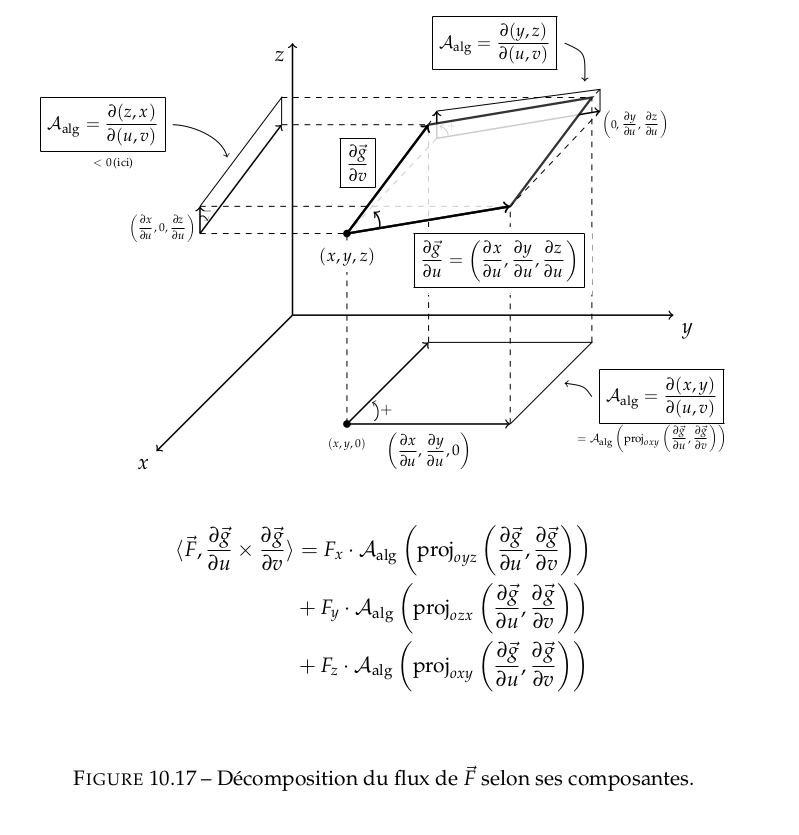
\includegraphics[scale=0.4]{images/MATH-H2000_10_17}
\end{center}
\subsubsection{Figure 10.28 -- Coordonnées polaires}
\begin{center}
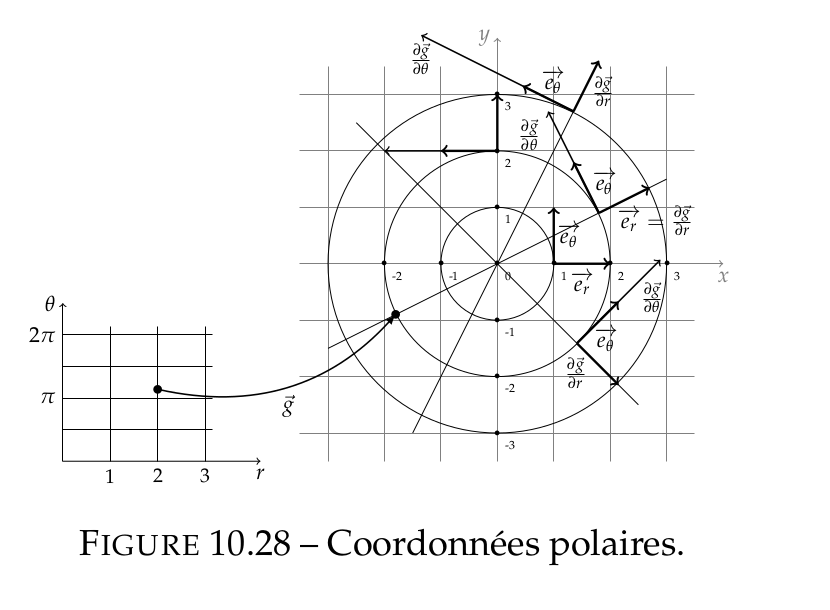
\includegraphics[scale=0.4]{images/MATH-H2000_10_28}
\end{center}
\subsubsection{Figure 10.44 -- Champ vectoriel et son rotationnel}
\begin{center}
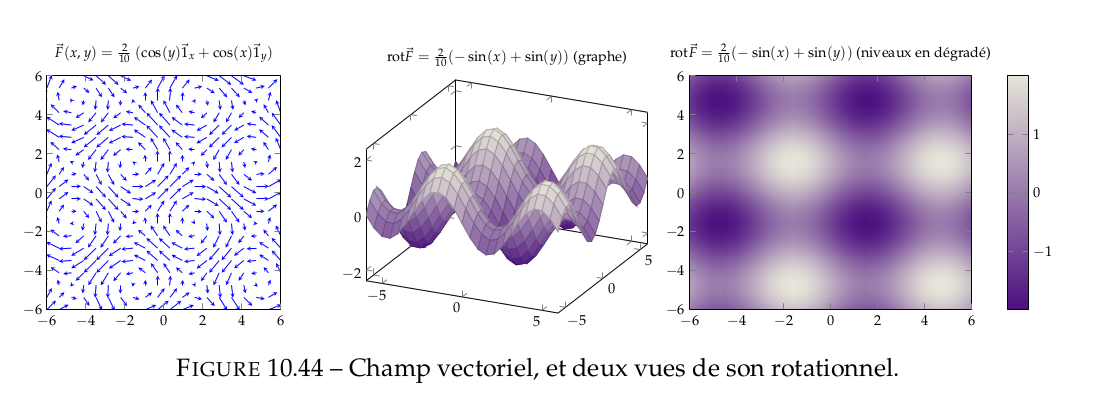
\includegraphics[scale=0.4]{images/MATH-H2000_10_44}
\end{center}



\section{Artem \textsc{Napov} -- MATH-H202 : Analyse numérique}
\subsection{Chapitre 3}
\subsubsection{Exemple 22 -- Représentation schématique de matrices}
\begin{center}
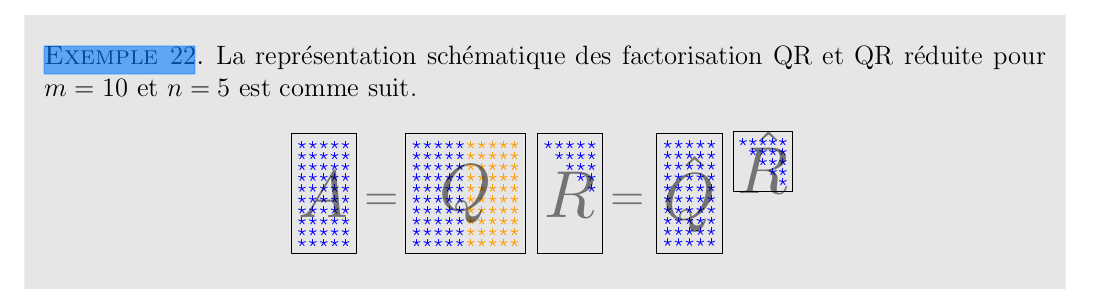
\includegraphics[scale=0.4]{images/MATH-H202_Exemple_22}
\end{center}
\subsection{Chapitre 5}
\subsubsection{Exemple 30 -- Zoom dans une illustration de la méthode de fausse position}
\begin{center}
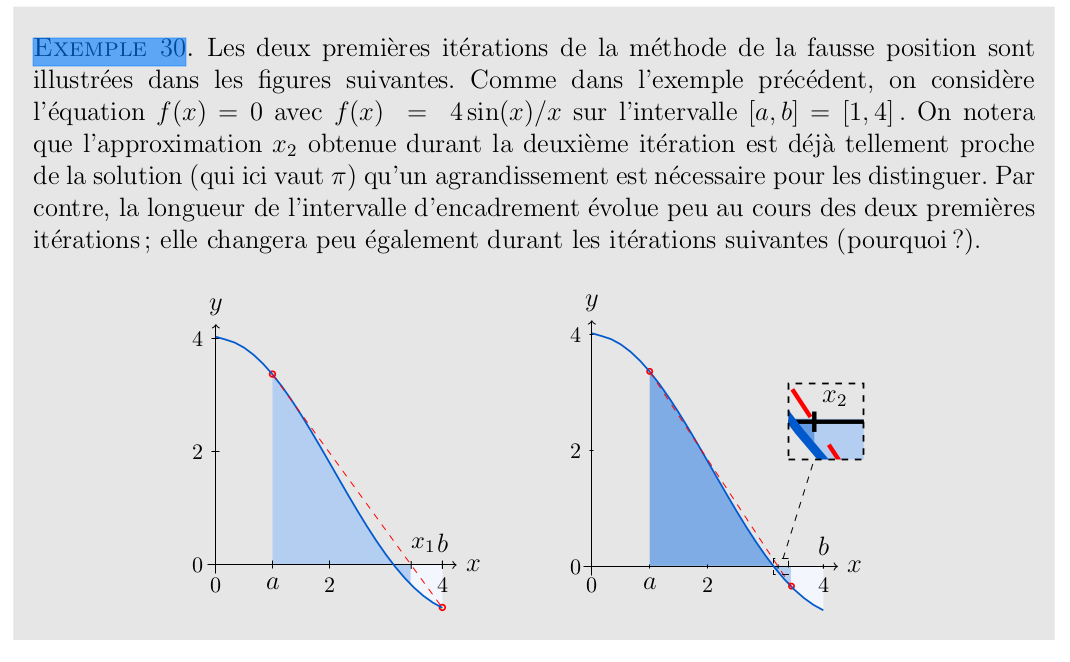
\includegraphics[scale=0.4]{images/MATH-H202_Exemple_30}
\end{center}

\subsection{Chapitre 7}
\subsubsection{Figures 7.1 et 7.2 -- Fonction, et aire de polygone}
\begin{center}
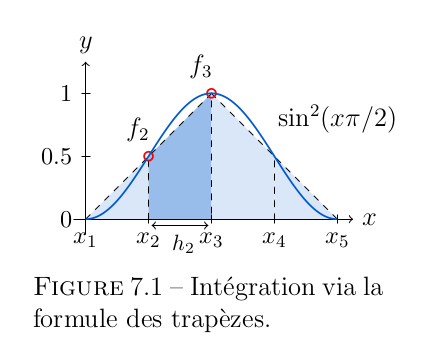
\includegraphics[scale=0.4]{images/MATH-H202_Figure_7_1}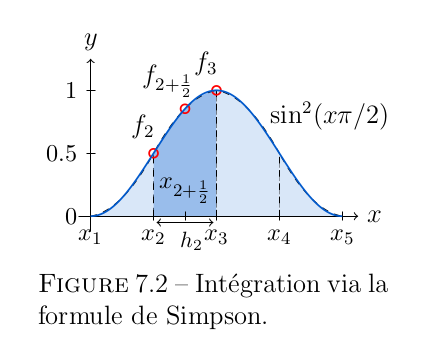
\includegraphics[scale=0.4]{images/MATH-H202_Figure_7_2}
\end{center}


\section{Jérémie \textsc{Roland} -- INFO-H304 : Compléments de programmation et d'algorithmique}
\subsection{Cours 5 -- Recherche de pic 1D : illustrations avec tableau}
\begin{center}
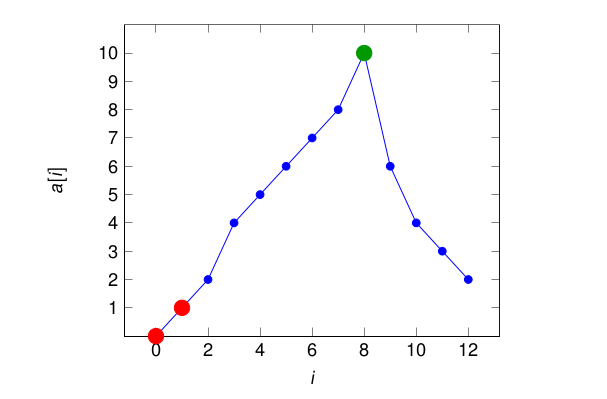
\includegraphics[scale=0.3]{images/INFO-H304_C5_1}
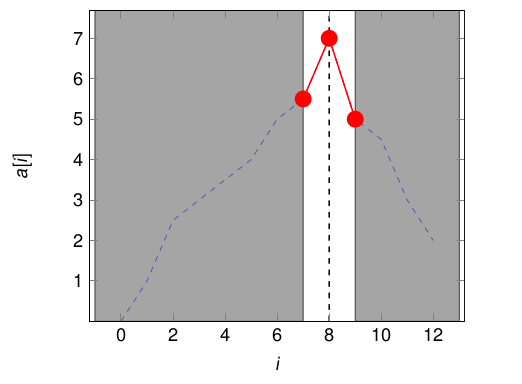
\includegraphics[scale=0.3]{images/INFO-H304_C5_2}
\end{center}
\subsection{Cours 6}
\subsubsection{Slide 42/51 : Arbre avec annotation, et tableau}
\begin{center}
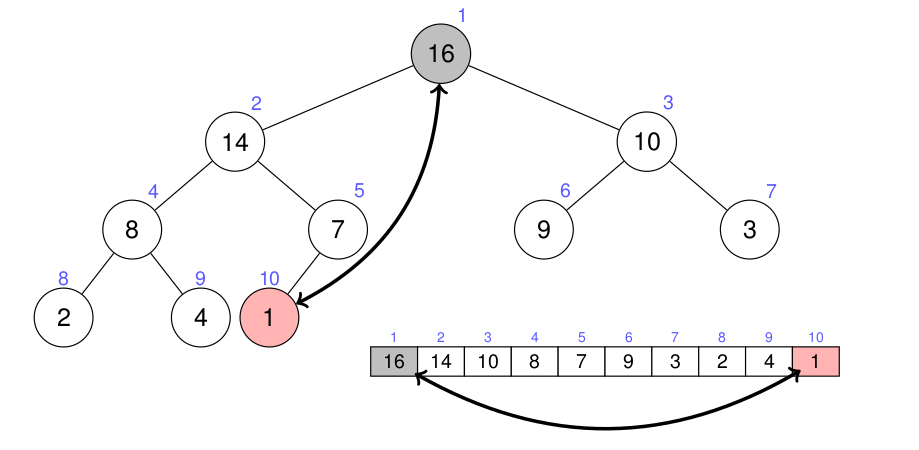
\includegraphics[scale=0.3]{images/INFO-H304_C6_1}
\end{center}
\subsubsection{Slide 40/51 : Arbre de récurrence avec annotation}
\begin{center}
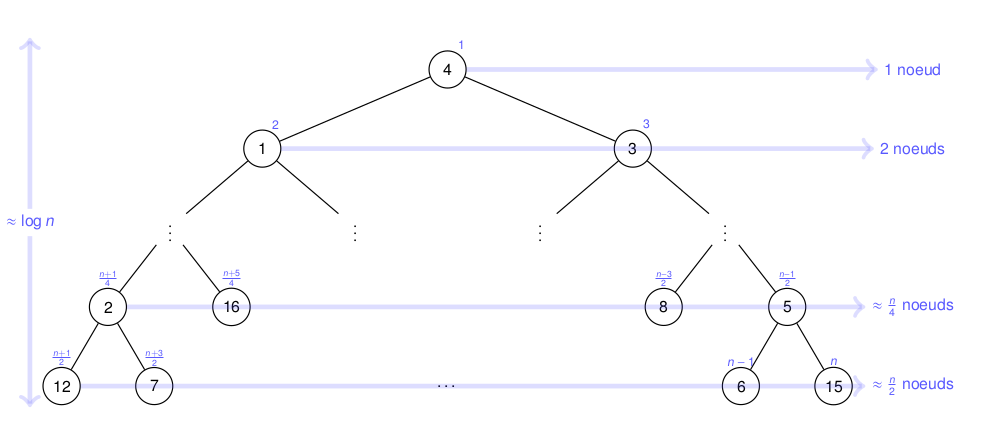
\includegraphics[scale=0.3]{images/INFO-H304_C6_2}
\end{center}
\subsection{Cours 7}
\subsubsection{Slide 27/77 : Arbre avec backtracking}
\begin{center}
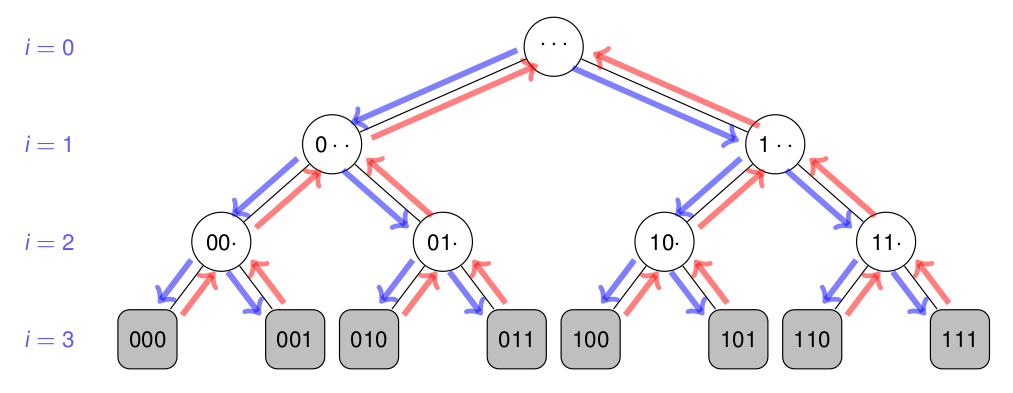
\includegraphics[scale=0.3]{images/INFO-H304_C7_1}
\end{center}
\subsubsection{Slide 35/77 : Problème du sac à dos}
\begin{center}
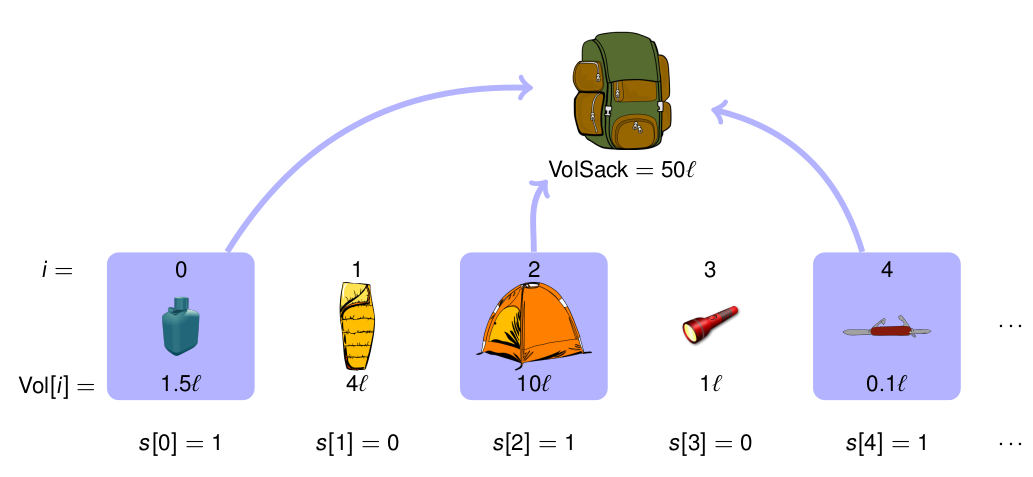
\includegraphics[scale=0.3]{images/INFO-H304_C7_2}
\end{center}
\subsubsection{Slide 49/77 : Manipulation d'un échiquier}
\begin{center}
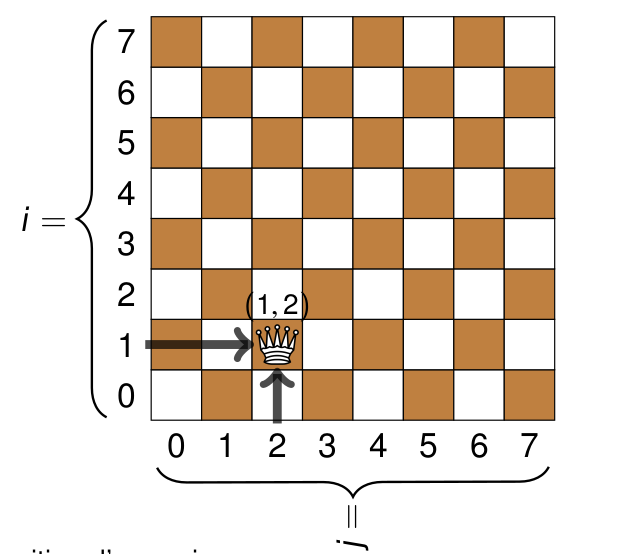
\includegraphics[scale=0.3]{images/INFO-H304_C7_3}
\end{center}
\subsection{Cours 9}
\subsubsection{Slide 40/43 : Arbre avec annotation (flèche, texte)}
\begin{center}
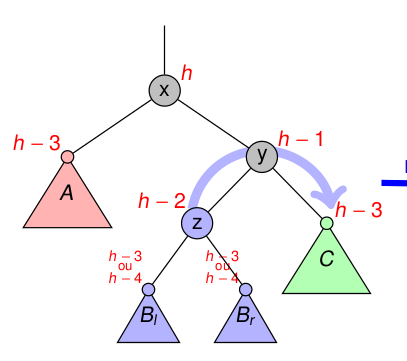
\includegraphics[scale=0.3]{images/INFO-H304_C9_1}
\end{center}
\subsection{Cours 9}
\subsubsection{Slide 16/49 : Liste chaînée, ensembles avec annotation}
\begin{center}
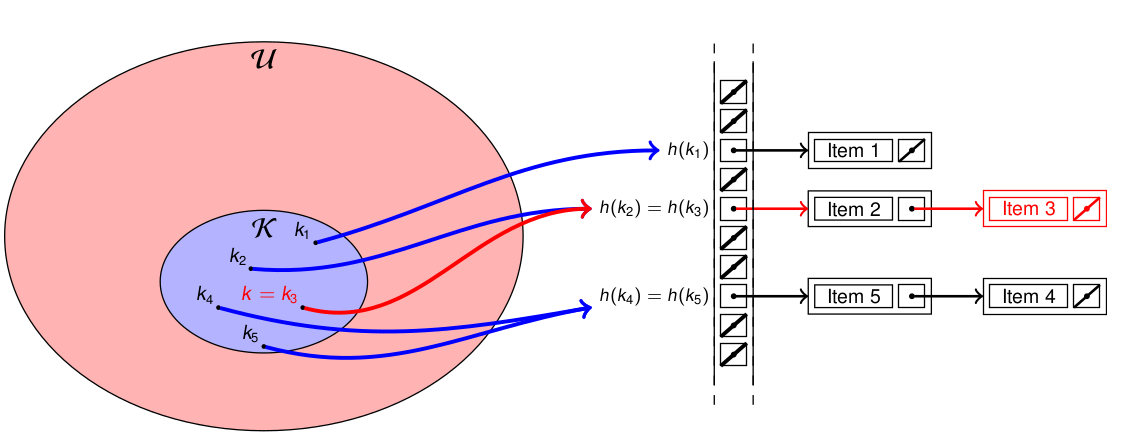
\includegraphics[scale=0.3]{images/INFO-H304_C10_1}
\end{center}
\subsubsection{Slide 22/49 : Opérations sur bits}
\begin{center}
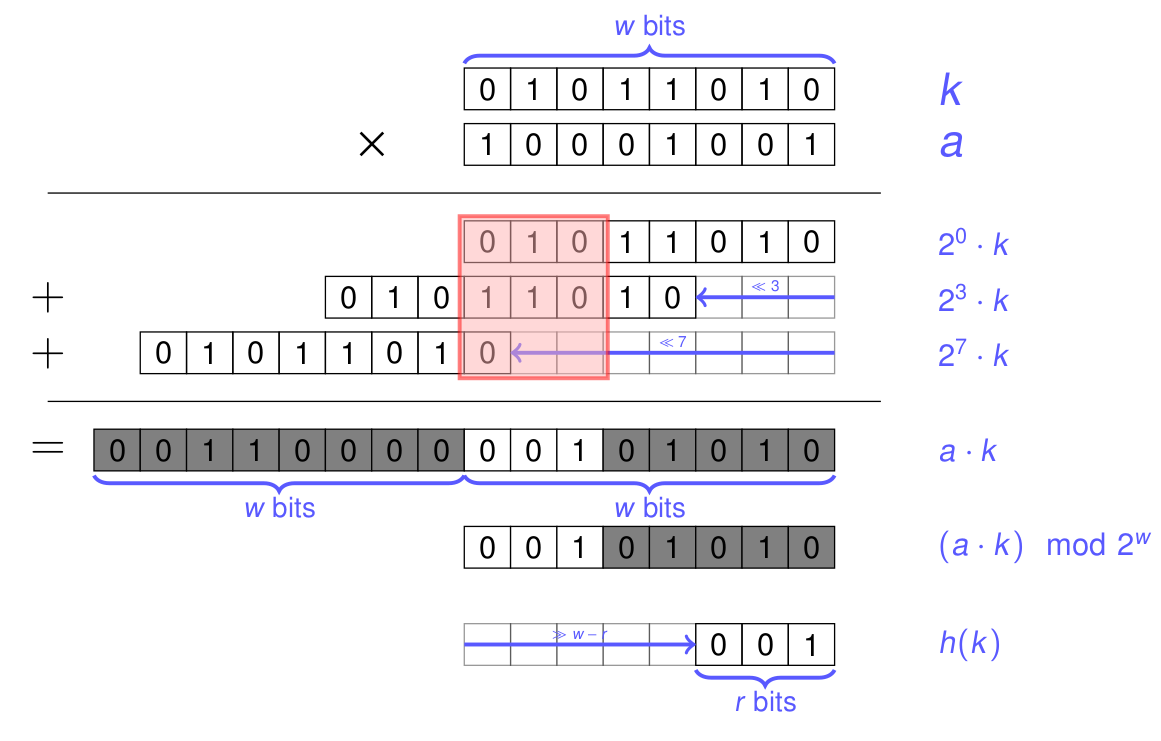
\includegraphics[scale=0.3]{images/INFO-H304_C10_2}
\end{center}
\subsection{Cours 12}
\subsubsection{Slide 46/71 : Problème du sac-à-dos fractionnel}
\begin{center}
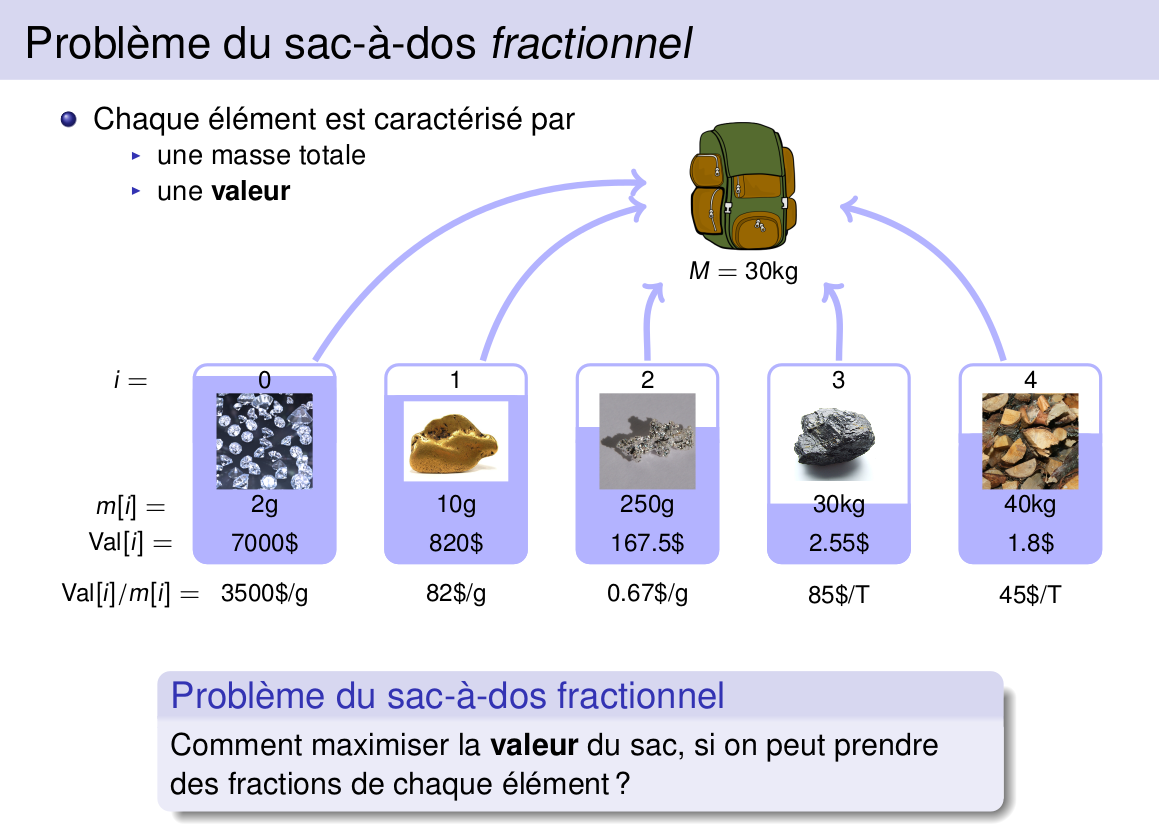
\includegraphics[scale=0.3]{images/INFO-H304_C12_1}
\end{center}
\subsubsection{Slide 61/71 : Graphe de dépendances}
\begin{center}
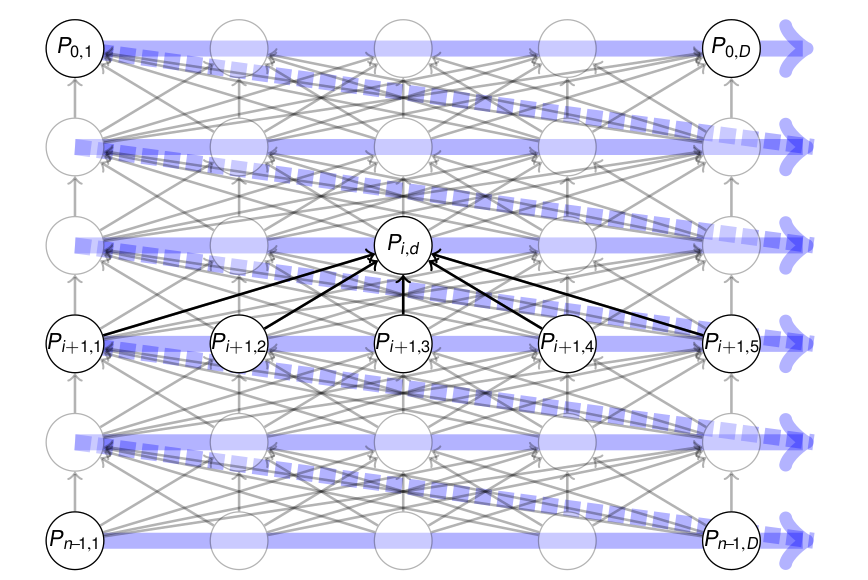
\includegraphics[scale=0.3]{images/INFO-H304_C12_2}
\end{center}
\end{document}